\documentclass{article}

\usepackage{graphicx}
\usepackage{tikz}
\usepackage{tikzsymbols}
\usetikzlibrary{calc,patterns,shapes.geometric}
\pagestyle{empty}
\usepackage[margin=0pt]{geometry}
\geometry{papersize={14in,12in}}

\def\centerarc[#1](#2)(#3:#4:#5){\draw[#1] ($(#2)+({#5*cos(#3)},{#5*sin(#3)})$) arc (#3:#4:#5);}

\begin{document}
	\begin{figure}
		\centering
		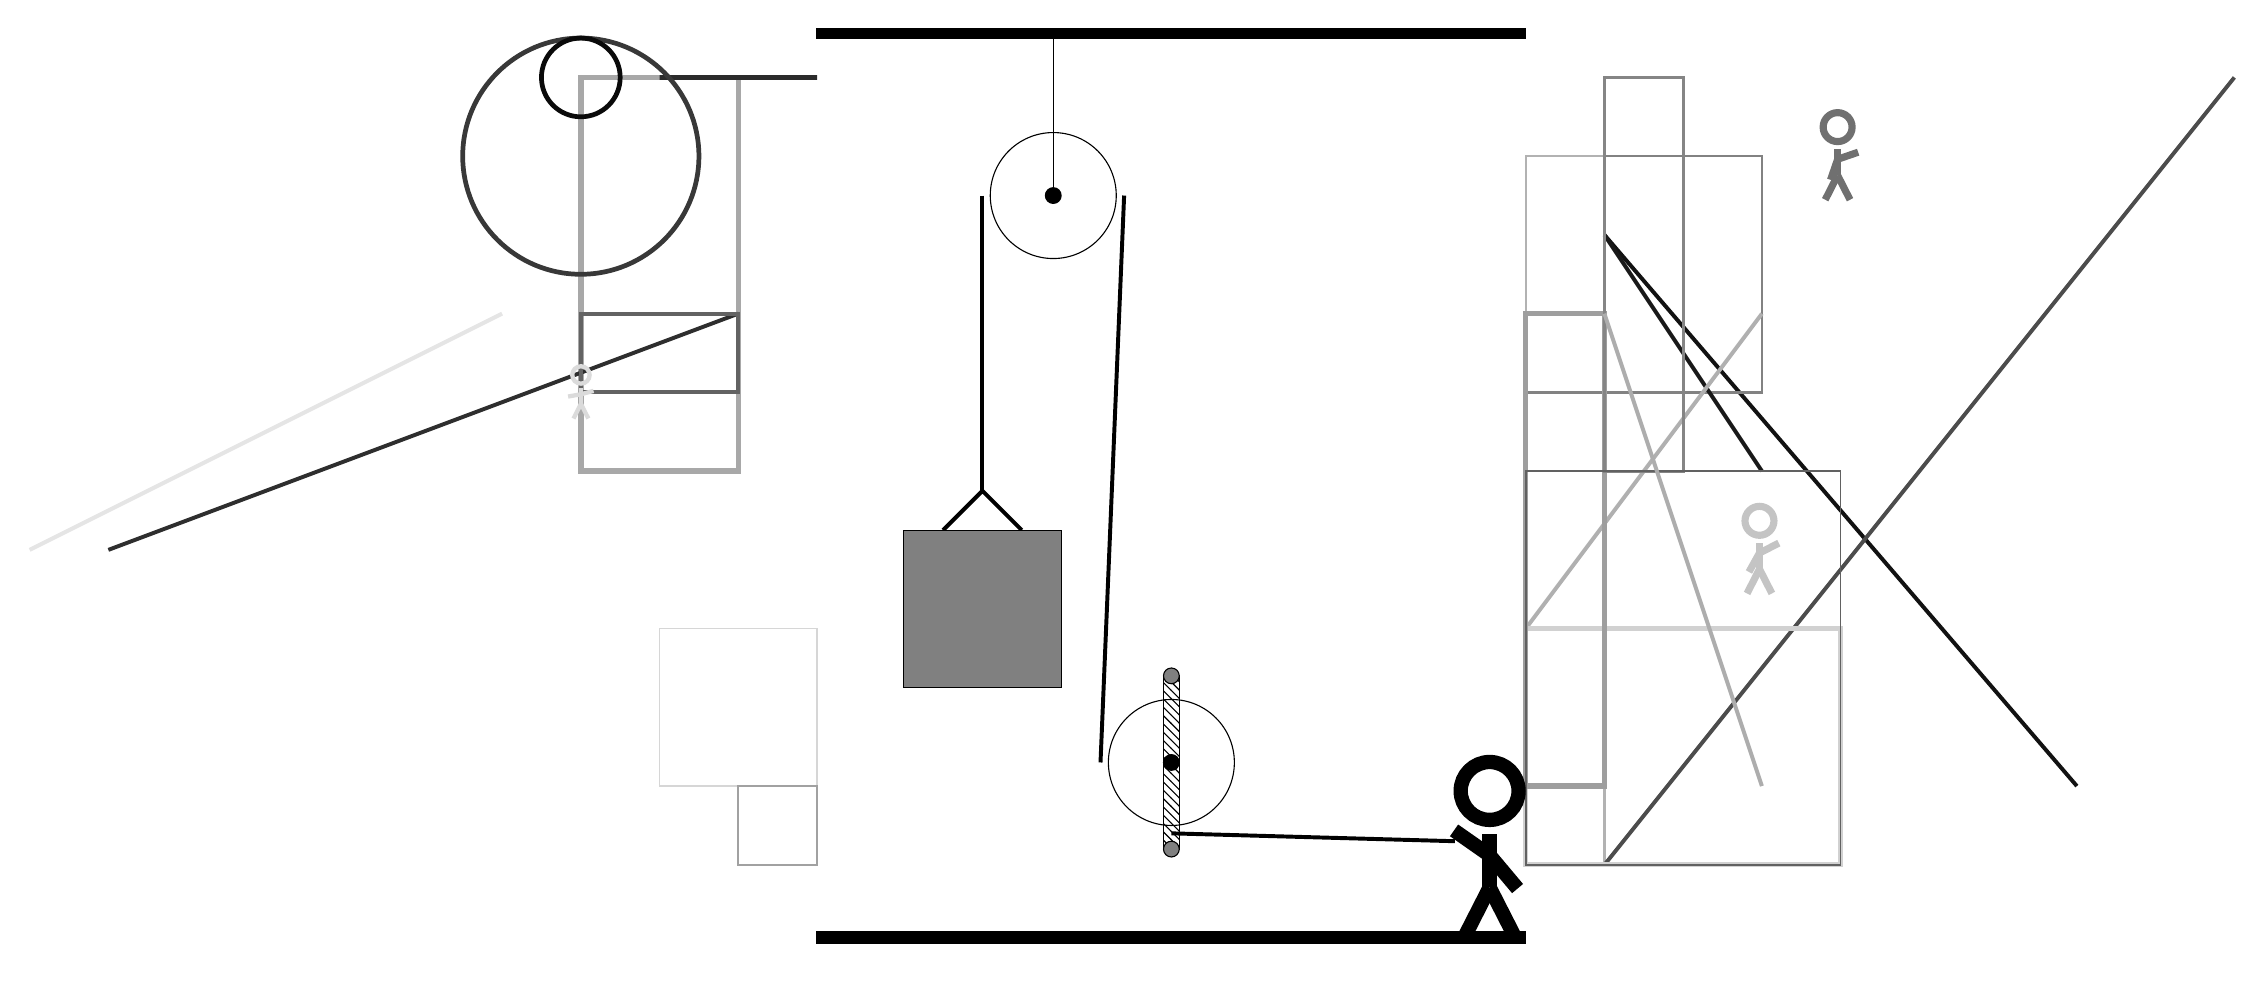
\begin{tikzpicture}
			%%%%% START %%%%%
			
			\draw[fill=black] (-2, 11.5) rectangle (7, 11.625);
			
			\draw (1, 9.5) circle (0.8);
			\draw[fill=black] (1, 9.5) circle (0.1);
			\draw (1, 11.5) -- (1, 9.5);
			
			\draw[line width=0.2mm, color=black!16] (-4, 2) rectangle (-2, 4);
			
			\draw[line width=0.7mm, color=black!34] (-3, 6) rectangle (-5, 11);
			\draw[line width=0.5mm, color=black!93](8, 9) -- (14, 2);
			\draw[line width=0.3mm, color=black!49] (7, 7) rectangle (10, 10);
			
			\draw[line width=0.5mm, color=black!82](-3, 8) -- (-11, 5);
			
			\draw[line width=0.7mm, color=black!83] (-2, 11) rectangle (-4, 11);
			\draw[line width=0.5mm, color=black!61] (-3, 8) rectangle (-5, 7);
			
			\draw[line width=0.3mm, color=black!30] (7, 1) rectangle (8, 10);
			\node[line width=0.3mm, color=black!14] at (-5, 7) {\Strichmaxerl[3][10][15]};
			
			\draw[line width=0.5mm, color=black!90](8, 9) -- (10, 6);
			\draw [line width=0.7mm, color=black!91](9, 4) circle (0.0);
			\draw [line width=0.6mm, color=black!78](-5, 10) circle (1.5);
			\draw[line width=0.5mm, color=black!10](-6, 8) -- (-12, 5);
			\draw[line width=0.5mm, color=black!31](10, 8) -- (7, 4);
			\draw[line width=0.5mm, color=black!70](8, 1) -- (16, 11);
			\draw[line width=0.6mm, color=black!18] (7, 4) rectangle (11, 1);
			\node[line width=0.4mm, color=black!56] at (11, 10) {\Strichmaxerl[5][71][19]};
			\draw[line width=0.3mm, color=black!37] (-3, 2) rectangle (-2, 1);
			\draw [line width=0.6mm, color=black!96](-5, 11) circle (0.5);
			\draw[line width=0.7mm, color=black!38] (8, 2) rectangle (7, 8);
			\draw[line width=0.4mm, color=black!48] (9, 6) rectangle (8, 11);
			
			\node[line width=0.3mm, color=black!23] at (10, 5) {\Strichmaxerl[5][61][27]};
			\draw[line width=0.2mm, color=black!62] (7, 1) rectangle (11, 6);
			\draw[line width=0.5mm, color=black!32](10, 2) -- (8, 8);
			
			\draw[fill=white](2.5, 2.3) circle (0.8);
			\draw[fill=black] (2.5, 2.3) circle (0.1);
			\draw[pattern=north west lines, pattern color=black] (2.4, 3.4) rectangle (2.6, 1.2);
			\draw[fill=black!50] (2.5, 3.4) circle (0.1);
			\draw[fill=black!50] (2.5, 1.2) circle (0.1);
			
			\draw[line width=0.5mm] (-0.4, 5.25) -- (0.1, 5.75) -- (0.6, 5.25);
			\draw[fill=black!50] (-0.9, 5.25) rectangle (1.1, 3.25);
			
			\draw[line width=0.5mm] (0.1, 9.5) -- (0.1, 5.75);
			\centerarc[line width=0.5mm](1, 9.5)(0:180:0.9);
			\draw[line width=0.5mm](1.9, 9.5) -- (1.6, 2.3);
			\centerarc[line width=0.5mm](2.5, 2.3)(180:270:0.9);
			\draw[line width=0.5mm](2.5, 1.4) -- (6.1, 1.3);
			
			\node at (6.5, 1.2) {\Strichmaxerl[10][-35][-50]};
			
			\draw[fill=black] (-2, 0) rectangle (7, 0.15);
			
			%%%%% END %%%%%
		\end{tikzpicture}
	\end{figure}	
\end{document}